%01 intro
\begin{frame}{Research Questions}	
	\begin{alertblockc}{}{jwigreige!100!white}%
		We \textbf{operationalize a novel measure} for the velocity of money \textbf{based on effectively circulation coins}.%
	\end{alertblockc}
	\begin{alertblockc}{}{jwilightgreen!90!white}%
		We test how well the simple \textbf{proxy-variables used so far} really are.%
	\end{alertblockc}
	\footnotetextNN{[Fisher, Irving: {T}he Equation of Exchange. 1911.]}
\end{frame}

\begin{frame}{``Velocity'' of money?}
	\vspace{1ex}
	\begin{alertblockc}[N]{}{jwimauve!80!white}%
		How are transactions executed using money?
	\end{alertblockc}
  \begin{figure}
    \centerline{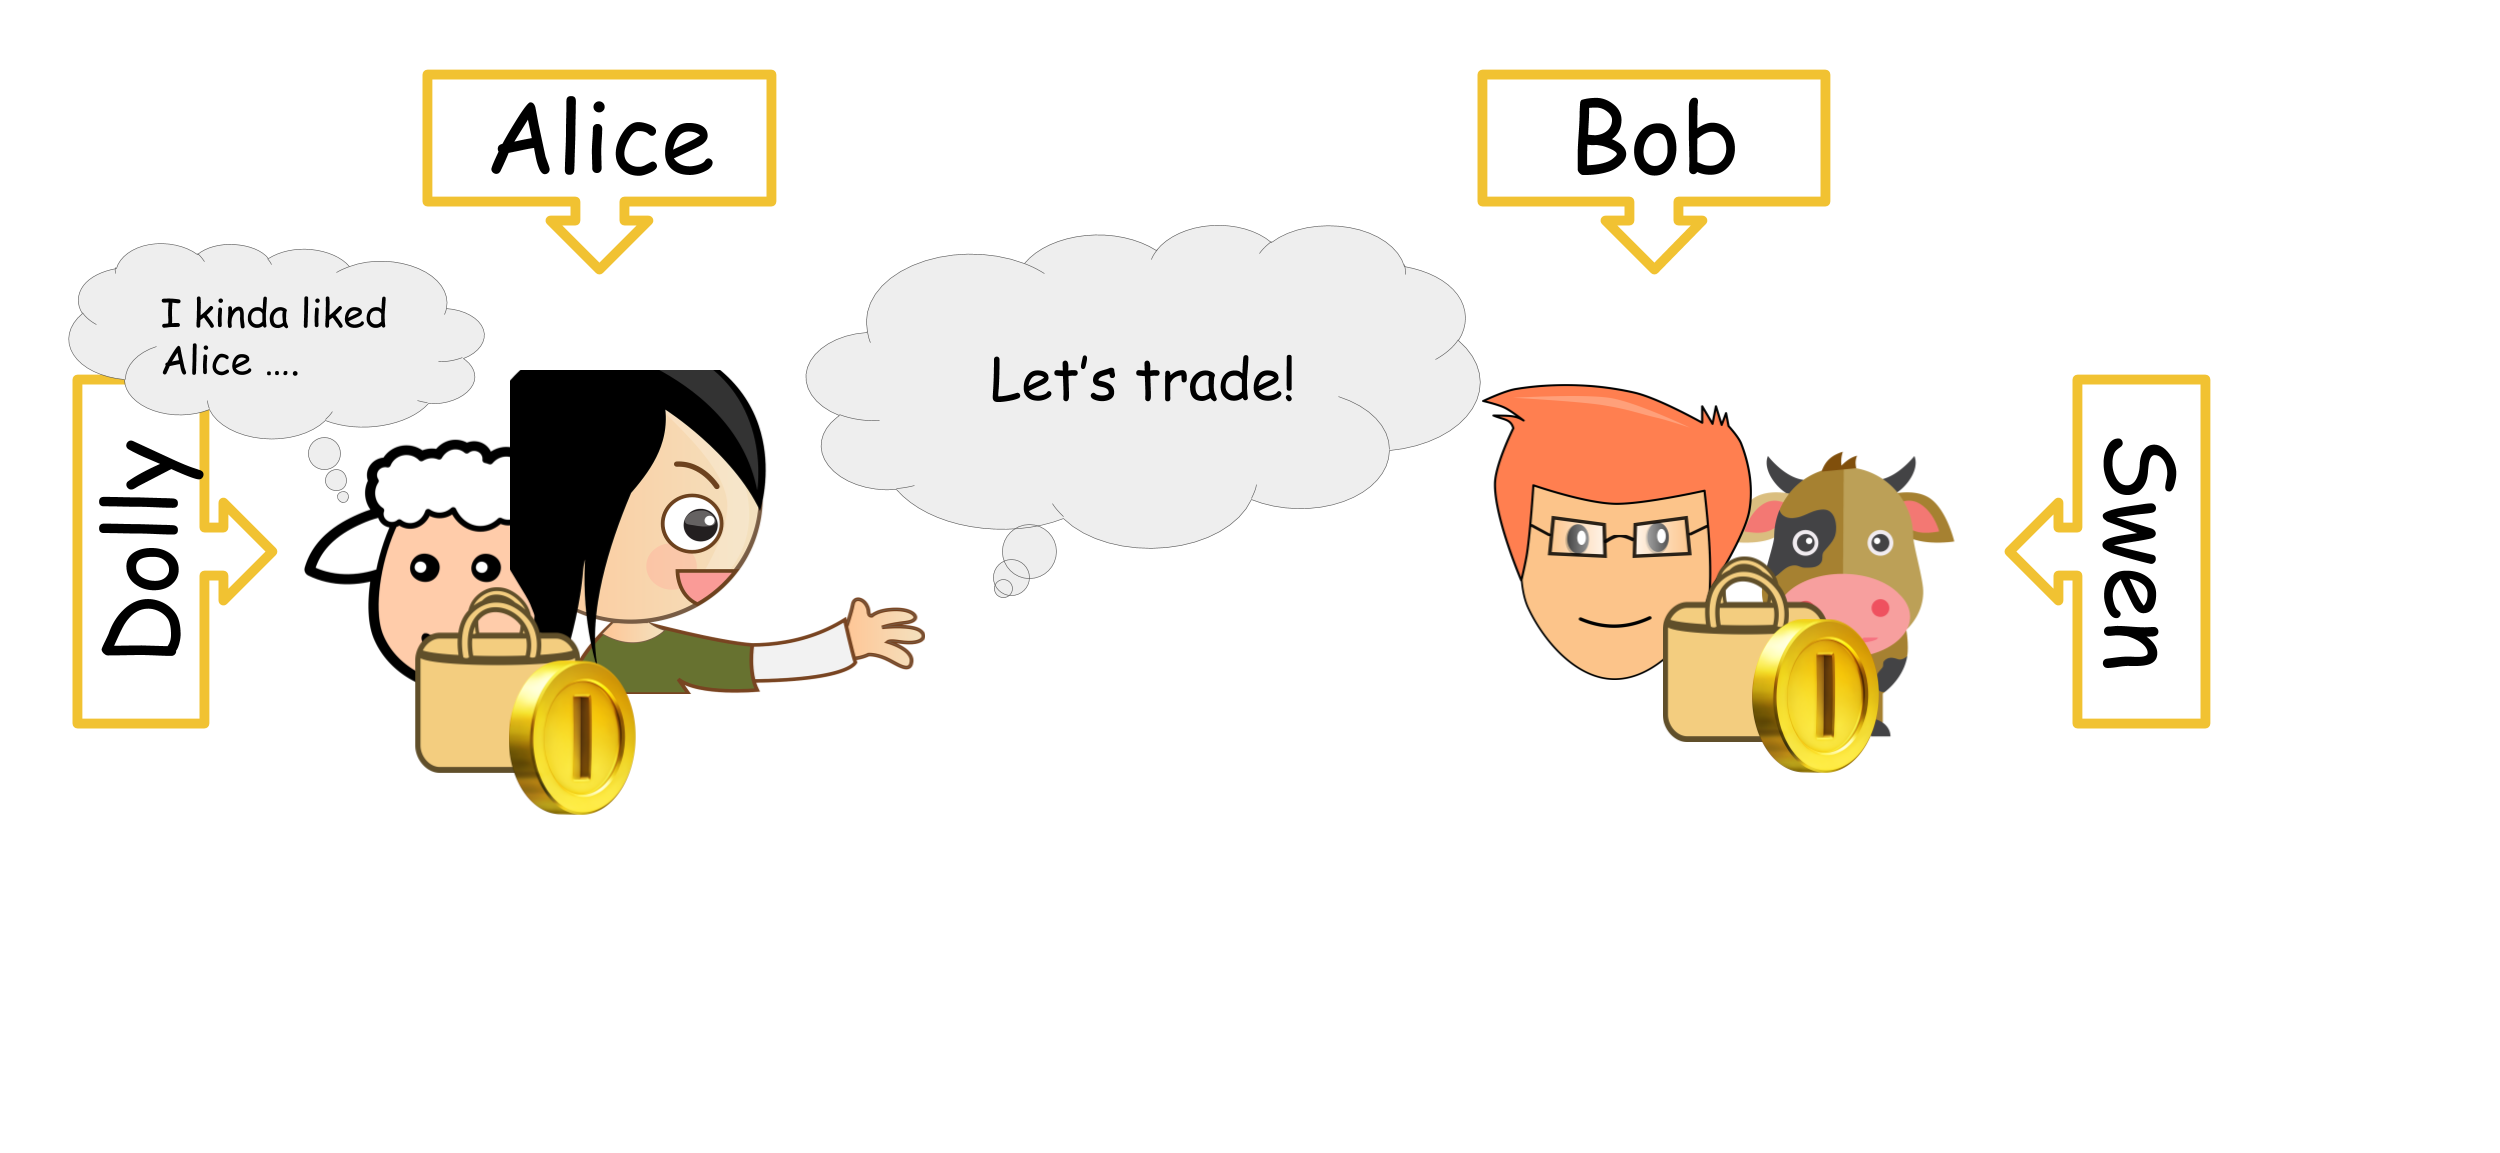
\includegraphics[scale=0.17]{./pics/used/sheep_example_intro_HR(2)}}
  \end{figure}
\end{frame}

\begin{frame}{``Velocity'' of money?}	
	\vspace{1ex}
	\begin{alertblockc}[N]{}{jwimauve!80!white}%
		How are transactions executed using money?
	\end{alertblockc}
	\vspace{0.5ex}
  \begin{figure}
    \centerline{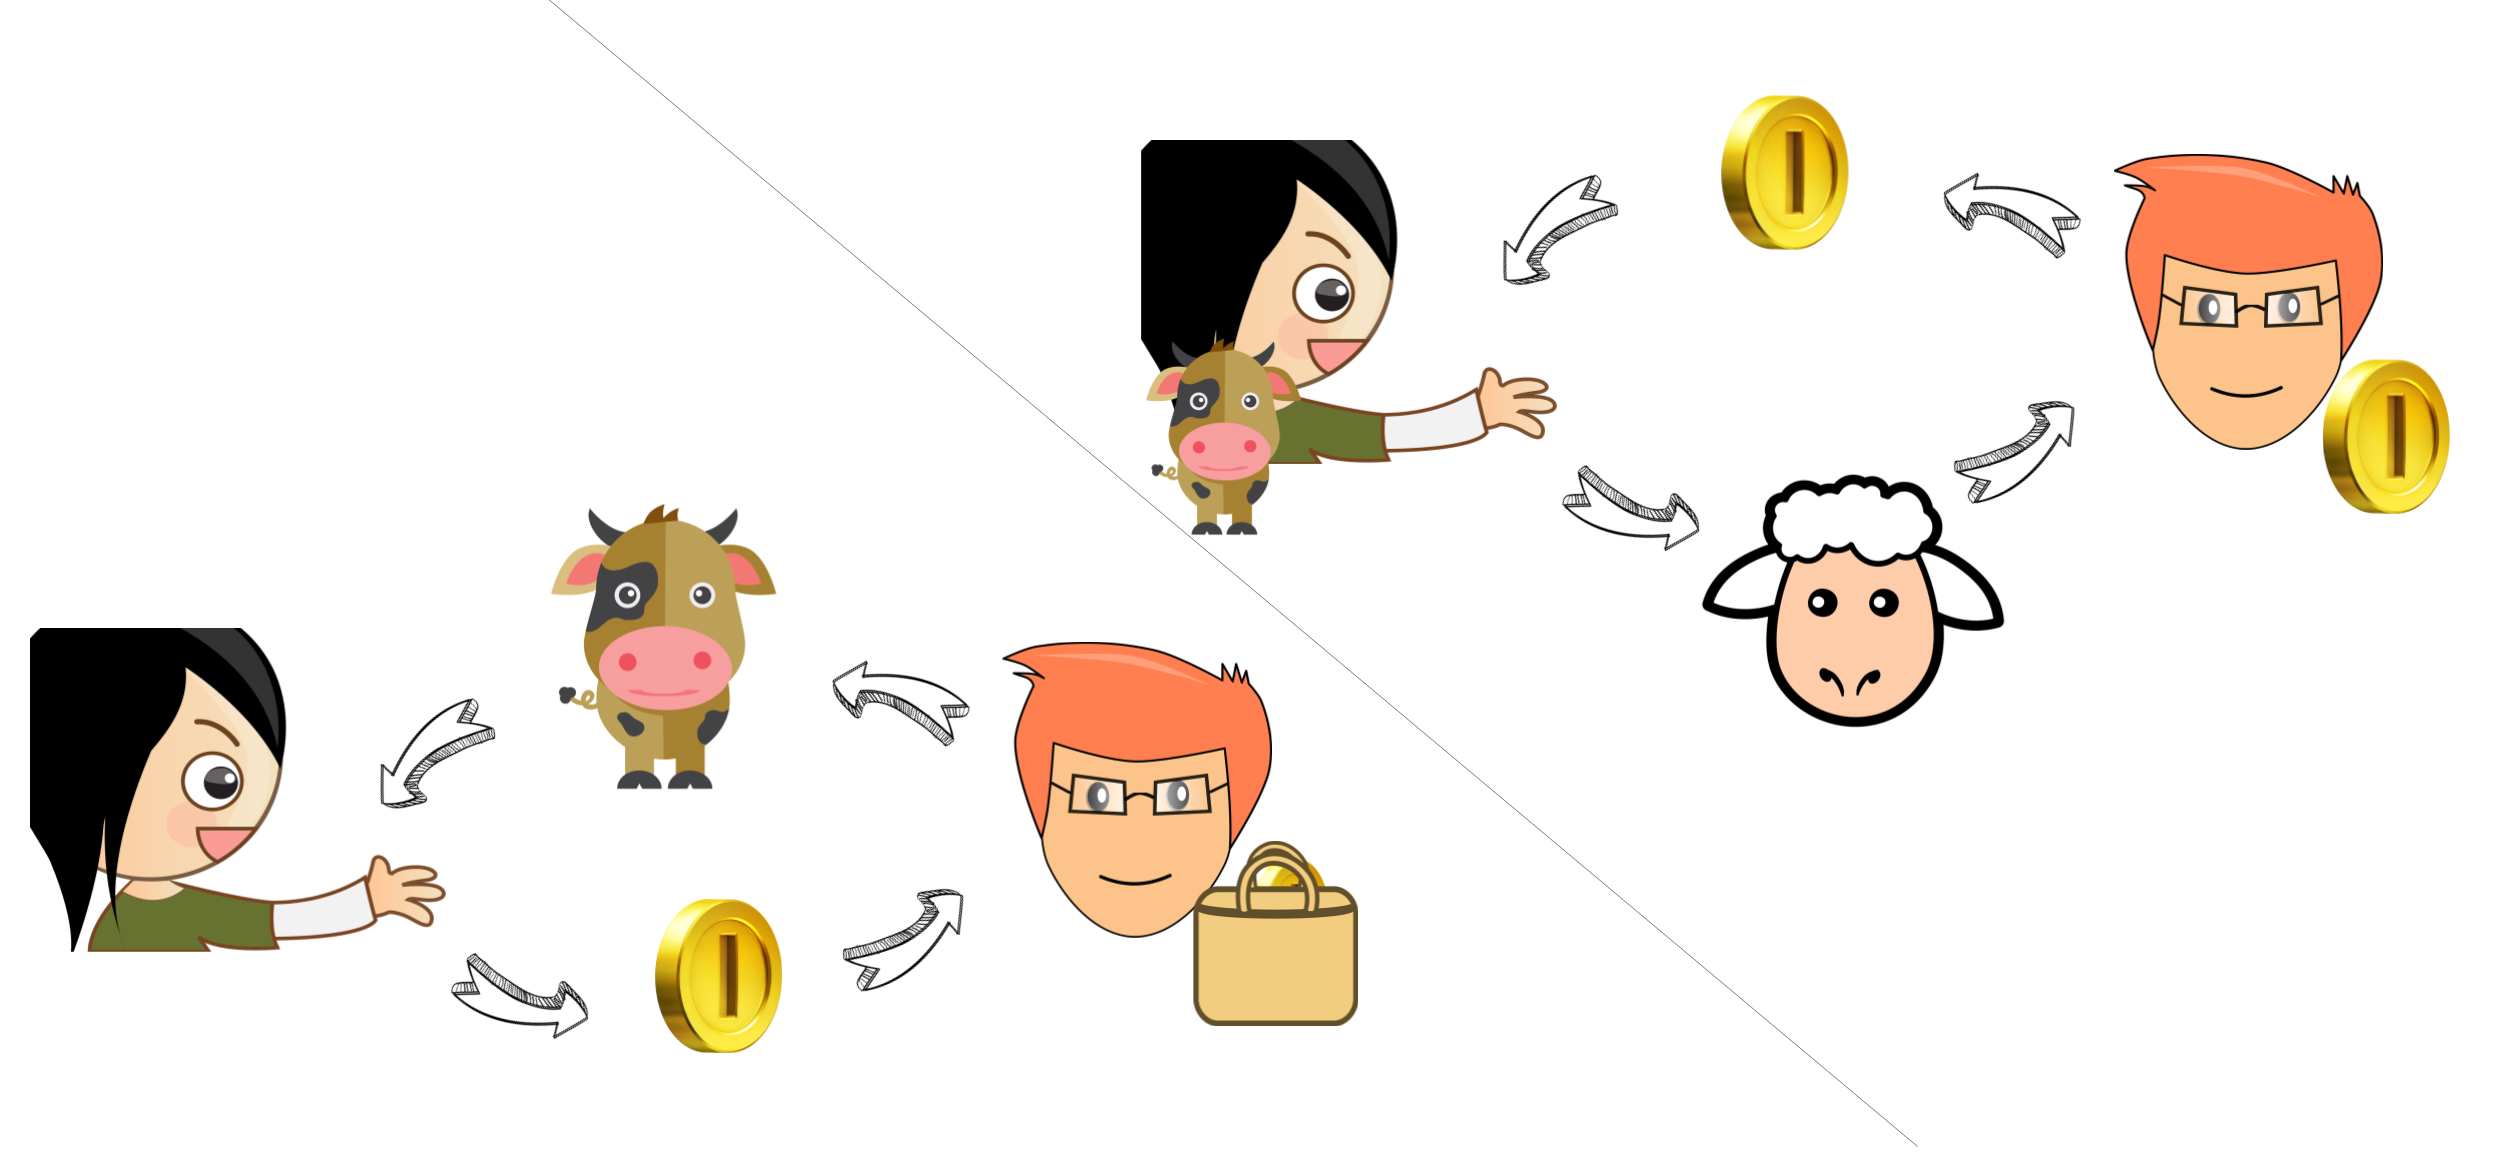
\includegraphics[scale=0.105]{./pics/used/sheep_example_intro_HR(3)}}
  \end{figure}
  \centering
  \vspace{-2em}
  \begin{align*}%
    \text{\textbf{T}ransaction volume} = %
    \Biggl\langle
    \underbrace{ 
      \renewcommand*{\arraystretch}{1.035}
      \begin{pmatrix}%
      1\,\frac{\coinsSmall}{\sheepSmall} \\%
      1\,\frac{\coinsSmall}{\cowSmall}%
    \end{pmatrix}
  }_{\text{\textbf{P}rice Vector}}
    , % 
    \underbrace{
      \renewcommand*{\arraystretch}{1.1}
      \begin{pmatrix}%
      1\,\sheep \\%
      1\,\cow%
    \end{pmatrix}
  }_{\text{\textbf{T}ransact. Vector}}
    \Biggr\rangle %
    = 2\,\coins
  \end{align*} %
  \\%	
\end{frame}

\begin{frame}{``Velocity'' of money?}
	\vspace{1ex}
	\begin{alertblockc}{}{jwimauve!80!white}%
		Can we still do the same deals with just one coin?
	\end{alertblockc}
  \begin{figure}
    \centerline{
\includegraphics[scale=0.15]{./pics/used/sheep_example_intro_HR(4)}}
  \end{figure}
\end{frame}

\begin{frame}{``Velocity'' of money?}
	\vspace{1ex}
	\begin{alertblockc}[N]{}{jwilightgreen!90!white}%
		Yes! We just spin the leftover coin for a second time within this period!%
	\end{alertblockc}
  \begin{figure}
    \centerline{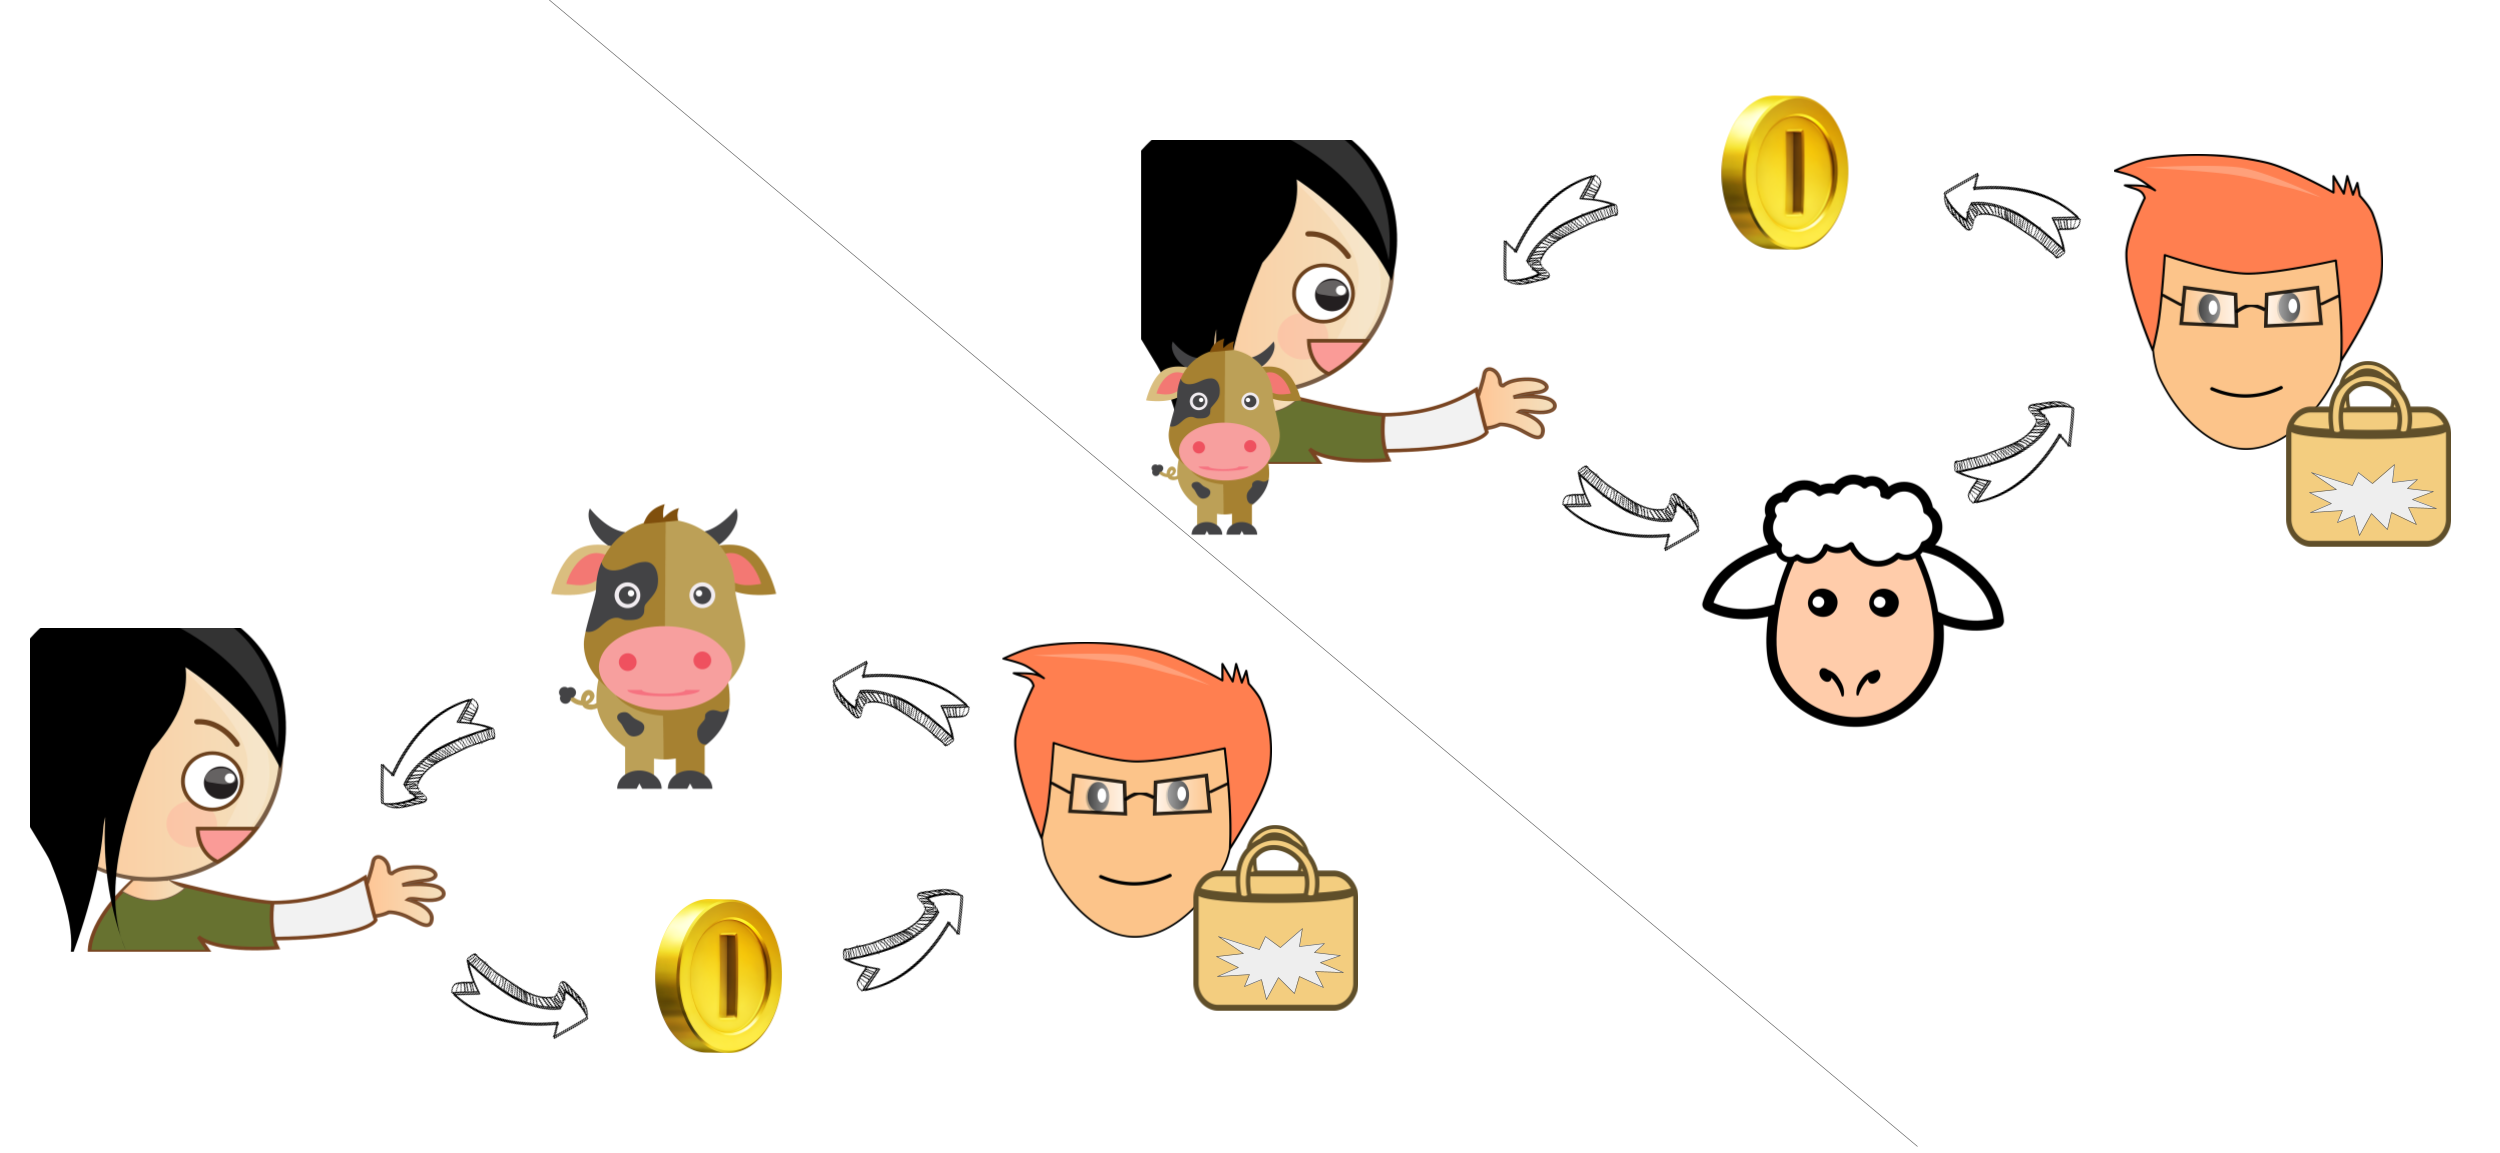
\includegraphics[scale=0.12]{./pics/used/sheep_example_intro_HR(5)}}
  \end{figure}
	\vspace{-1.5em}
	\begin{alertblockc}{}{jwimauve!80!white}%
		How does this work?
	\end{alertblockc}
\end{frame}





